\documentclass[12pt]{article}

% a template that a friend gave, it's worked well enough for me
% i have added some packages and stuff that have proved useful

\usepackage{fancyhdr}
\usepackage{tipa}
\usepackage{fontspec}
\usepackage{amsfonts}
\usepackage{enumitem}
\usepackage[margin=1in]{geometry}
\usepackage{graphicx}
\usepackage{float}
\usepackage{amsmath}
\usepackage{braket}
\usepackage{amssymb}
\usepackage{booktabs}
\usepackage{hyperref}
\usepackage{mathtools}
\usepackage{xcolor}
\usepackage{float}
\usepackage{algpseudocodex}
\usepackage{titlesec}
\usepackage{bbm}

\pagestyle{fancy}
\fancyhf{} % sets both header and footer to nothing
\lhead{Kevin Sheng}
\setmainfont{Comic Neue}
\renewcommand{\headrulewidth}{1pt}
\setlength{\headheight}{0.75in}
\setlength{\oddsidemargin}{0in}
\setlength{\evensidemargin}{0in}
\setlength{\voffset}{-.5in}
\setlength{\headsep}{10pt}
\setlength{\textwidth}{6.5in}
\setlength{\headwidth}{6.5in}
\setlength{\textheight}{8in}
\renewcommand{\headrulewidth}{0.5pt}
\renewcommand{\footrulewidth}{0.3pt}
\setlength{\textwidth}{6.5in}
\usepackage{setspace}
\usepackage{multicol}
\usepackage{float}
\setlength{\columnsep}{1cm}
\setlength\parindent{24pt}
\usepackage [english]{babel}
\usepackage [autostyle, english = american]{csquotes}
\MakeOuterQuote{"}

\setlength{\parskip}{6pt}
\setlength{\parindent}{0pt}

\titlespacing\section{0pt}{12pt plus 4pt minus 2pt}{0pt plus 2pt minus 2pt}
\titlespacing\subsection{0pt}{12pt plus 4pt minus 2pt}{0pt plus 2pt minus 2pt}
\titlespacing\subsubsection{0pt}{12pt plus 4pt minus 2pt}{0pt plus 2pt minus 2pt}

\hypersetup{colorlinks=true, urlcolor=blue}

\newcommand{\correction}[1]{\textcolor{red}{#1}}


\rhead{ECE 102}

\newcommand{\rect}{\operatorname{rect}}

\begin{document}

\begin{enumerate}
      \item \begin{enumerate}
                  \item Yes, the system is linear.
                        \begin{align*}
                              S(ax(t)+w(t))
                               & = \cos(t)(ax(t)+w(t))          \\
                               & = a(\cos(t) x(t))+\cos(t) w(t) \\
                               & = aS(x(t))+S(w(t))\quad\square
                        \end{align*}
                  \item No, the system is not linear.
                        \begin{align*}
                              S(ax(t)) & = ax'(t) \cdot (ax(t))^2 \\
                                       & = a^3 x'(t) \cdot x(t)^2 \\
                              aS(x(t)) & = a x'(t) \cdot x(t)^2   \\
                                       & \ne S(ax(t))
                        \end{align*}
                        From this, we can see that the homogeneity principle does not hold.
                  \item No, the system is not linear.
                        \begin{align*}
                              S(ax(t)) & = e^{ax(t)}               \\
                                       & = \left(e^{x(t)}\right)^a \\
                              aS(x(t)) & = ae^{x(t)}               \\
                                       & \ne S(ax(t))
                        \end{align*}
            \end{enumerate}
      \item \begin{enumerate}
                  \item Notice that $x_2(t)=x_1(t)+x_1(t+1)$.
                        Since the system is LTI, the response is $y_1(t)+y_1(t+1)$.

                        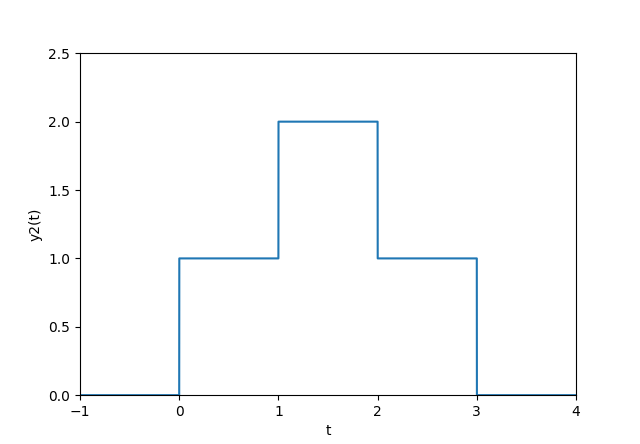
\includegraphics[width=12cm]{img/hw3/a}
                  \item We want to figure out the output if the system if the input is $\delta(t)$.
                        \begin{align*}
                              a^t \cos t
                               & = \int_{-\infty}^{\infty} u(\tau) h(t-\tau)\,d\tau \\
                               & = \int_{0}^{\infty} h(t-\tau)\,d\tau
                        \end{align*}
                        After some trial and error, we can find that
                        \[h(t)=a^t(\ln a \cos t - \sin t)\]
                        To get the desired system output, we calculate $0.5(h(t+1)+h(t-1))$:
                        \[0.5\left(a^{t+1}(\ln a \cos (t+1) - \sin (t+1))+a^{t-1}(\ln a \cos (t-1) - \sin (t-1))\right)\]

                        Since $\exists t < 0: h(t) \ne 0$, the system isn't causal.
            \end{enumerate}
      \item \begin{enumerate}
                  \item \begin{enumerate}
                              \item I found it easier to calculate $g * f$.
                                    \begin{align*}
                                          (g * f)(t)
                                           & = \int_{-\infty}^{\infty} e^{-\tau}u(\tau)(\delta(t-\tau+1)+5\delta(t-\tau-2))\,d\tau                      \\
                                           & = \int_{0}^{\infty} e^{-\tau}(\delta(t-\tau+1)+5\delta(t-\tau-2))\,d\tau                                   \\
                                           & = \int_{0}^{\infty} e^{-\tau}\delta(t-\tau+1)\,d\tau + 5\int_{0}^{\infty} e^{-\tau}\delta(t-\tau-2)\,d\tau \\
                                           & = \boxed{e^{-(t+1)}u(t+1)+5e^{-(t-2)}u(t-2)}
                                    \end{align*}
                              \item \begin{align*}
                                          (f * g)(t)
                                           & = \int_{-\infty}^{\infty} 2\rect \left(\tau-\frac{3}{2}\right) \cdot 2r(t-\tau-1)\rect\left(t-\tau-\frac{3}{2}\right)\,d\tau \\
                                           & = 4\int_{1}^{2} r(t-\tau-1)\rect\left(t-\tau-\frac{3}{2}\right)\,d\tau                                                       \\
                                           & = 4\int_{1}^{2} (t-\tau-1)\rect\left(t-\tau-\frac{3}{2}\right)\,d\tau
                                    \end{align*}
                                    This integral can be broken down into three cases:
                                    \[(f * g)(t)=\begin{cases}
                                                0                               & t < 2       \\
                                                4\int_{1}^{t-1} t-\tau-1\,d\tau & 2 \le t < 3 \\
                                                4\int_{t-2}^{2} t-\tau-1\,d\tau & 3 \le t < 4 \\
                                                0                               & t > 4
                                          \end{cases}\]
                                    Simplifying the middle two integrals gives us
                                    \[(f * g)(t)=\begin{cases}
                                                0            & t < 2       \\
                                                2(t-2)^2      & 2 \le t < 3 \\
                                                -2t^2+12t-16 & 3 \le t < 4 \\
                                                0            & t > 4
                                          \end{cases}\]
                        \end{enumerate}
                  \item Consider $h(t)=(u(t)-u(t-T))t^2$.
                        Our convolution is then
                        \begin{align*}
                              (x * h)(t)
                               & = \int_{-\infty}^{\infty} x(\tau)h(t-\tau)\,d\tau                  \\
                               & = \int_{-\infty}^{\infty} x(\tau)(u(t-\tau)-u(t-\tau-T))(t-\tau)^2
                        \end{align*}
                        For the middle term to be nonzero, we need $t-\tau \ge 0$ and $t-\tau-T \le 0$.
                        Simplifying and combining these two inequalities gives us $t-T \le \tau \le t$, so
                        \[\int_{-\infty}^{\infty} x(\tau)(u(t-\tau)-u(t-\tau-T))(t-\tau)^2
                              =\int_{t-T}^{t} x(\tau)(t-\tau)^2\,d\tau\]
                  \item \begin{enumerate}
                              \item We can swap the order of the summation
                                    and integral to turn it into an infinite geometric series.
                                    \begin{align*}
                                          e^t * \sum_{k=0}^{\infty} \delta(t-k)
                                           & = \int_{-\infty}^{\infty} e^\tau \sum_{k=0}^{\infty} \delta(t-k-\tau)\,d\tau \\
                                           & = \sum_{k=0}^{\infty} \int_{-\infty}^{\infty} e^\tau \delta(t-k-\tau)\,d\tau \\
                                           & = \sum_{k=0}^{\infty} e^{t-k}                                                \\
                                           & = \boxed{\frac{e^{t+1}}{e-1}}
                                    \end{align*}
                              \item In accordance with the hint, we first evaluate $u(t)*u(t)$:
                                    \begin{align*}
                                          u(t) * u(t)
                                           & = \int_{-\infty}^{\infty} u(\tau)u(t-\tau)\,d\tau \\
                                           & = \int_{0}^{\infty} u(t-\tau)\,d\tau              \\
                                           & = r(t)
                                    \end{align*}
                                    Now, we use the properties of convolution to do the following:
                                    \begin{align*}
                                          (u(t)-u(t-1))*u(t-2)       & = u(t)*u(t-2)-u(t-1)*u(t-2) \\
                                                                     & = r(t-2)-r(t-3)             \\
                                          \frac{d}{dt} r(t-2)-r(t-3) & = \boxed{u(t-2)-u(t-3)}
                                    \end{align*}
                        \end{enumerate}
            \end{enumerate}
      \item \begin{enumerate}
                  \item I propose $h_1(t)=e^{-3t}u(t)$.
                        \begin{align*}
                              (x*h_1)(t)
                               & = \int_{-\infty}^{\infty} x(\tau)e^{-3(t-\tau)}u(t-\tau)\,d\tau \\
                               & = \int_{\infty}^{t} x(\tau) e^{-3(t-\tau)}\,d\tau
                        \end{align*}
                        which is our desired convolution.
                  \item 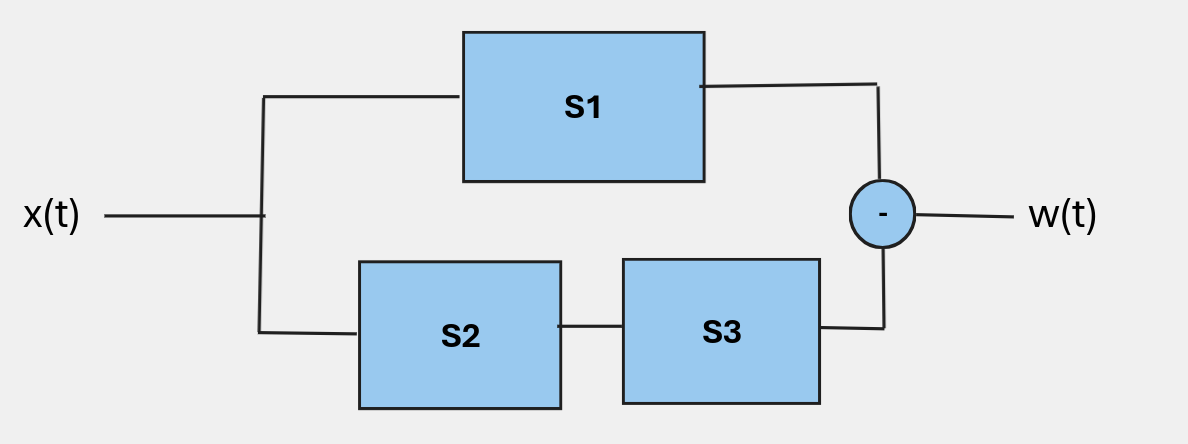
\includegraphics[width=12cm]{img/hw3/chain}
                  \item We already figured out the impulse response of $\mathcal{S}_1$.
                        It remains to figure out $h_2$.
                        I propose $h_2=u(t-2)$.
                        Then,
                        \begin{align*}
                              (x*h_2)
                               & = \int_{-\infty}^{\infty} x(\tau) u(t-2-\tau)\,d\tau \\
                               & = \int_{-\infty}^{t-2} x(\tau)\,d\tau
                        \end{align*}
                        To get $\mathcal{S}_3(h_2(x))$, we take $h_2 * h_3$:
                        \begin{align*}
                              (h_2 * h_3)
                               & = \int_{-\infty}^{\infty} u(\tau - 2) \delta(t-\tau-3)\,d\tau \\
                               & = \int_{2}^{\infty} \delta(t-\tau-3)\,d\tau                   \\
                               & = u(t-5)
                        \end{align*}
                        Now, we subtract this from $h_1$ to get
                        \[h_1(x)-(h_2 * h_3)(x)=\boxed{e^{-3t}u(t)-u(t-5)}\]
                  \item The given input signal can be decomposed into a linear combination of impulses:
                        \begin{align*}
                              \mathcal{S}_{eq}(\delta(t)+2\delta(t-3))
                               & = h_{eq}(t)+2h_{eq}(t-3)                                    \\
                               & = e^{-3t}u(t)-u(t-5)+2\left(e^{-3(t-3)}u(t-3)-u(t-8)\right)
                        \end{align*}
            \end{enumerate}
      \item After this PDF will be the Jupyter Notebook I ran.
\end{enumerate}
\end{document}
